\section{Upgrade Plans for Long Shutdown 1 and Beyond}

During long shutdown 1 (LS1) it has been decided to first carry out measurements of the beam impedance and electrical breakdowns tests of the proposed new beam screen design, and subsequently upgrade 8 kicker magets implementing the new screen design and the additional proposed changes to the inside of the vacuum tank to reduce the temperatures reached in the ferrite yoke. Thermal simulations have indicated that the proposed screen design will be capable of reducing the maximum temperature reached in the ferrite yoke below the curie temperature for the nominal operating conditions for the LHC, and for a number of proposed HL-LHC operating conditions also (see Fig.~\ref{fig:pow-loss-stable-temp-mkis}). In addition electric field simulations have strongly indicated that the transient electric field on the inner surfce of the ceramic tube, associated with the screen conductors, will not be sufficient to induce surface flashover. 


\begin{figure}
\begin{center}
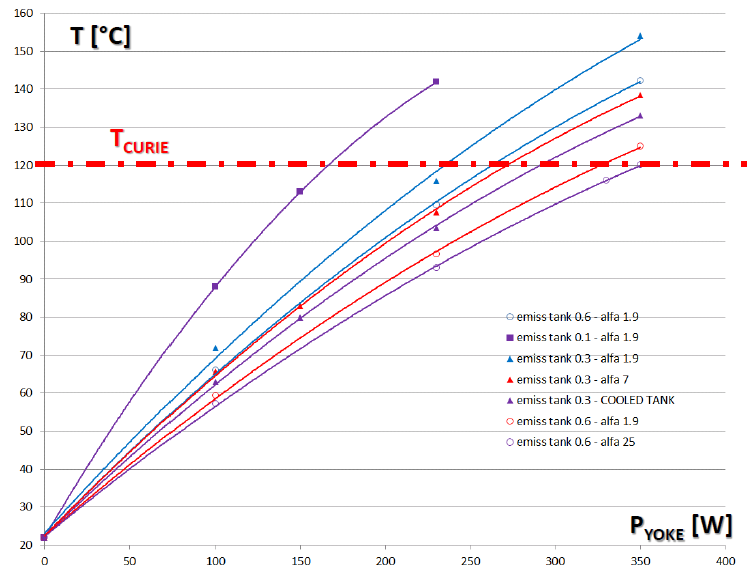
\includegraphics[width=0.8\textwidth]{LHC_MKI/figures/tempPowMarco.png}
\end{center}
\caption{The maximum steady-state temperature reached by the ferrite yoke in the MKI depending on the power load in the ferrite yoke as calculated using a 2D cross section of the MKI. $P_{yoke}$ is the power lost in the ferrite yoke and T the maximum steady state temperature of the ferrite yoke. Provided by M. Garlasche et al \cite{Garlasche:2dHeatEmisAll}.}
\label{fig:pow-loss-stable-temp-mkis}
\end{figure} 

Further monitoring of the MKIs will be necessary, as the stored current in the LHC is increased, due to possible further sources of heating within the magnets. However the work done on the understanding of the beam impedance, the heat transfer within the magnet and the electric field during kicker pulsing has greatly improved the knowledge of possible limitations in the future and the variety of solutions/counter measures that may be implemented. 